\begin{explanationbox}
	\textbf{\textcolor{CExplanation}{为什么要比较增长快慢？}}
	有的题目同时出现$2^x$、$x^{10}$和$\log_2x$。直接代入一个很大的数太麻烦；如果知道谁\textbf{最终占优势}，就能迅速判断大小或分式的变化方向。

	\medskip
	\textbf{\textcolor{CExplanation}{最直观的办法：让$x$连续翻倍}}
	先取最容易算的一组：$2^x$、$x^2$、$\log_2x$。
	\begin{center}
	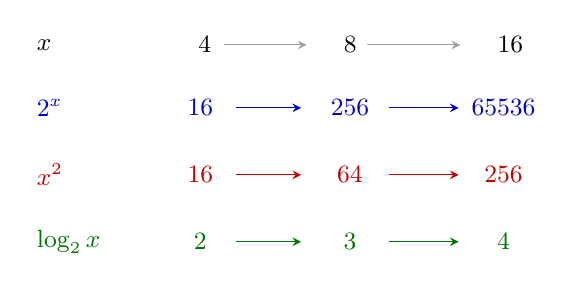
\begin{tikzpicture}[x=1cm,y=1cm,>=stealth,font=\small]
		\node[anchor=west] at (0,3.0) {$x$};
		\node[anchor=west] at (2.05,3.0) {$4$};
		\node[anchor=west] at (3.9,3.0) {$8$};
		\node[anchor=west] at (5.85,3.0) {$16$};
		\draw[->,gray!75] (2.5,3.0)--(3.55,3.0);
		\draw[->,gray!75] (4.32,3.0)--(5.5,3.0);
		\node[anchor=west,blue!75!black] at (0,2.2) {$2^x$};
		\node[blue!75!black] at (2.2,2.2) {$16$};
		\node[blue!75!black] at (4.1,2.2) {$256$};
		\node[blue!75!black] at (6.05,2.2) {$65536$};
		\draw[->,blue!75!black] (2.65,2.2)--(3.48,2.2);
		\draw[->,blue!75!black] (4.6,2.2)--(5.48,2.2);
		\node[anchor=west,red!75!black] at (0,1.35) {$x^2$};
		\node[red!75!black] at (2.2,1.35) {$16$};
		\node[red!75!black] at (4.1,1.35) {$64$};
		\node[red!75!black] at (6.05,1.35) {$256$};
		\draw[->,red!75!black] (2.65,1.35)--(3.48,1.35);
		\draw[->,red!75!black] (4.6,1.35)--(5.48,1.35);
		\node[anchor=west,green!45!black] at (0,0.5) {$\log_2x$};
		\node[green!45!black] at (2.2,0.5) {$2$};
		\node[green!45!black] at (4.1,0.5) {$3$};
		\node[green!45!black] at (6.05,0.5) {$4$};
		\draw[->,green!45!black] (2.65,0.5)--(3.48,0.5);
		\draw[->,green!45!black] (4.6,0.5)--(5.48,0.5);
	\end{tikzpicture}

	\end{center}
	\begin{description}[style=nextline,leftmargin=2.8em,labelsep=0.5em,itemsep=0.35em]
		\item[\textbf{指数：把原来的数再平方。}]
			$x$变成$2x$，$2^x$就变成$(2^x)^2$。例如$16\to256\to65536$，越往后越惊人。
		\item[\textbf{平方：每次只变成原来的$4$倍。}]
			$(2x)^2=4x^2$。例如$16\to64\to256$。
		\item[\textbf{对数：每次只增加$1$。}]
			$\log_2(2x)=\log_2x+1$。例如$2\to3\to4$。
	\end{description}
	这里让$x$\textbf{同样翻倍}，就容易看出为什么三者会拉开距离。

	\medskip
	\textbf{\textcolor{CExplanation}{从例子走向一般情况}}
	\begin{itemize}[leftmargin=*,itemsep=0.35em]
		\item 把$2$换成任何固定的$a>1$，即使$a$非常接近$1$，$a^x$最终也会超过$x^\alpha$。
		\item 把平方换成任何固定的$\alpha>0$，即使$\alpha$很小，$x^\alpha$最终也会超过$\log_ax$。
		\item $\log_ax$不是“不增长”，只是增长得很慢；它仍会随着$x$增大而不断增大。
	\end{itemize}

	\medskip
	\textbf{\textcolor{CExplanation}{考试什么时候最快用？}}
	分式里，\textbf{分子增长明显更快}，比值最终会越来越大；\textbf{分母增长明显更快}，比值会越来越接近$0$。注意先检查$a>1$、$\alpha>0$以及$x\to+\infty$这三个条件。
\end{explanationbox}
